\documentclass[11pt]{article}
\usepackage[margin=1in]{geometry}
\usepackage[T1]{fontenc}
\usepackage{lmodern}
\usepackage{amsmath,amssymb}
\usepackage{booktabs}
\usepackage{graphicx}
\usepackage{xcolor}
\usepackage[numbers,sort&compress]{natbib}
\usepackage[colorlinks=true,linkcolor=blue!50!black,citecolor=blue!50!black,urlcolor=blue!50!black]{hyperref}

% Every number in this paper is a macro generated by results/study3/make_study3_paper.py from seed_summary.json
% and suite_detection.json. Tables are generated the same way.
% Generated by results/study3/make_study3_paper.py from seed_summary.json. Do not edit by hand.
\newcommand{\ThrSelMean}{0.244}
\newcommand{\ThrSelSD}{0.116}
\newcommand{\ThrSelLo}{0.122}
\newcommand{\ThrSelHi}{0.366}
\newcommand{\ThrHeldMean}{0.064}
\newcommand{\ThrHeldSD}{0.157}
\newcommand{\ThrHeldLo}{-0.101}
\newcommand{\ThrHeldHi}{0.229}
\newcommand{\ThrRepK}{6}
\newcommand{\ThrRepLo}{0.541}
\newcommand{\ThrRepHi}{1.000}
\newcommand{\ThrTransferK}{1}
\newcommand{\ThrTrLo}{0.004}
\newcommand{\ThrTrHi}{0.641}
\newcommand{\ThrTransferAllK}{2}
\newcommand{\ThrTrAllLo}{0.028}
\newcommand{\ThrTrAllHi}{0.600}
\newcommand{\ThrSelPosAll}{8}
\newcommand{\ThrGapPosAll}{6}
\newcommand{\ThrDetLoopVone}{14.5}
\newcommand{\ThrDetLoopVtwo}{69.7}
\newcommand{\ThrDetMapVone}{35.6}
\newcommand{\ThrDetMapVtwo}{99.7}
\newcommand{\ThrMissLoopVtwo}{30.3}

\newcommand{\repo}{\url{https://github.com/abdelkabirouadoukou/si-loop}}

\title{Guarded Self-Improvement with a Live Language-Model Proposer:\\[2pt] Replication, Transfer, and Two Judge Defects}
\author{Abdelkabir Ouadoukou\thanks{Independent researcher. Contact: abdelkabir.ouadoukou@gmail.com.
Substantial AI assistance was used; see the disclosure at the end.}}
\date{November 2026}

\begin{document}
\maketitle
\vspace{-1.2em}

\begin{abstract}
Study~2 showed that a guarded self-improvement loop, with a sealed judge and a two-stage gate, rejects bad patches when the proposer is a script.
Study~3 replaces the script with a live language model (\texttt{openai/gpt-oss-120b}, JSON mode, temperature $0.7$) and asks three questions:
does the model's proposal stream produce patches that the gate accepts, does this repeat across independent replicates, and do accepted patches transfer to a family that selection never sees.
We run the solver-only arm (the model may edit one library file and sees its source and docstrings, never the hidden tests) in six pre-registered replicates (seeds 4 to 9).
Every replicate produced at least one accepted patch on the correctness path. The mean gain on the sealed selection families was $\ThrSelMean$ (95\% t-interval $[\ThrSelLo,\ThrSelHi]$), and no final evaluation contained a broken problem, meaning one that the anchor solved and the final champion fails.
Transfer to the held-out parsing family was rare. One of six replicates met the pre-declared generalisation criterion, which needs four. Across the nine seeded runs, two showed a held-out gain, and both came from one docstring-based fix to \texttt{roman\_to\_int}.
The transfer rate is $\ThrTransferAllK$ of $9$ (exact 95\% interval $[\ThrTrAllLo,\ThrTrAllHi]$), so we do not claim generalisation.
Two defects in our own judge surfaced during the study. A gate clause was always true and admitted a patch that did not improve the library (D1). A verifier suite missed a tie-break bug in \texttt{two\_sum} (D2), and its miss rate depends strongly on which bug the model writes.
We report both defects, the deviations they forced, and the measurements that followed, and we keep the pilot run in the record.
\end{abstract}

\section{Introduction}

Study~2 \citep{ouadoukou2026study2} built the kernel for guarded self-improvement: a two-stage paired gate, a margin budget against creeping degradation, a held-out family against adaptive overfitting, and a sealed verifier whose secret the agent cannot read.
Its proposer, however, was a script with a fixed list of fixes. The script could be tested without an API, and it showed that the machinery works, but it said nothing about whether a language model's proposals behave the same way.
Study~1 \citep{ouadoukou2026study1} reported that an over-cautious judge can look useless when it rejects most rounds, and that a rising curve does not by itself show that improving the improver helped.

The question here is narrower than recursive self-improvement. We ask whether a live model, given only the source and docstrings of a small library, produces patches that the same gate accepts on fresh problems, and whether those patches generalise across families.
The answer determines whether the improver arm of Study~4 is worth building on this kernel.

\paragraph{Contributions.} This paper makes four contributions.
\begin{itemize}\setlength\itemsep{1pt}
\item A live proposer with the kernel's strict parser, a hidden-test-free workspace reader, coarse feedback, and budget caps, evaluated against the unchanged sealed judge (Section~\ref{sec:system}).
\item A pre-registered replication design with six independent replicates, a declared primary test (transfer to the held-out family), and pre-declared verdict rules (Section~\ref{sec:prereg}).
\item Two defects in our own judge, each found by inspecting results, with the deviations they forced, a repaired gate clause, and a measured detection rate for the verifier suite (Section~\ref{sec:defects}).
\item Results that are mixed in the way the design predicts: local optimisation repeats, transfer does not (Section~\ref{sec:results}).
\end{itemize}

\section{System under test}
\label{sec:system}

The kernel is the one from Study~2. Only the proposer changes. The proposer is \texttt{LLMMetaAgent} (\texttt{kernel/llm\_meta.py}). It sends the model a prompt containing the current \texttt{agent/} source with comments stripped, a list of coarse outcomes for earlier proposals, and an instruction to return one JSON object of edit operations. The reply goes through the same strict parser as scripted proposals, and a malformed reply is retried with its error message, up to two times.

\paragraph{What the model sees.} The reader exposes only \texttt{agent/**}. Hidden tests, oracles, expected values, per-family numbers, pass counts and held-out results never reach the prompt. Source text is wrapped as untrusted data, so comments and strings cannot issue instructions. The history file records every proposal and its coarse verdict (accept, stepping stone, or reject, with an error type), and the model sees only that summary.
The prompt is capped at 12,000 characters, a reply at 1,500 tokens, and a proposal at eight edit hunks. A cycle may make at most three calls, with at least three seconds between calls, and is limited to 20,000 tokens. A run is capped at 200,000 tokens.

\paragraph{Judge and gate.} The judge is Study~2's \texttt{PytestVerifier}. Problem identifiers are HMACs under a random per-folder secret, so every batch is fresh. Candidate code runs in a sandbox process that receives inputs only. A separate process runs a hidden pytest file against the outputs.
The gate compares the candidate with its parent on paired problems. Let $b$ be the number of problems the candidate fixes, $c$ the number it breaks, and $n$ the batch size. The paired effect is $\delta=(b-c)/n$, with standard error $\sqrt{b+c-(b-c)^2/n}/n$. The reported lower bound is $\delta-1.645\,\mathrm{SE}$. The correctness path accepts only when $\delta>0$ and the exact one-sided probability $p=\Pr[\mathrm{Bin}(b+c+1,\tfrac12)\le b]$ is at least $p_{\mathrm{improve}}=0.95$. The first stage screens on batch A at threshold $0.80$. The second stage confirms on an independent batch B with $n=48$ problems. The two stages remove the winner's curse, because a patch must succeed on data its own screen did not see.
The false-discovery monitor is e-LOND \citep{xu2024elond}. In these runs it ran in monitor mode, so it logged its alarms and did not block anything.

\paragraph{Scope.} Arm A0 is the only arm run here. The model may edit \texttt{agent/lib.py}, and nothing else. The improver arms (A1, A3) are declared in the pre-registration and reserved for Study~4.

\section{Pre-registration and design}
\label{sec:prereg}

The pre-registration is \texttt{results/study3/prereg.json}. It records the model, the configuration, the hashes of the three files that define the run, the kernel digest, the deviations, and the analysis rules. Its body is hashed with SHA-256 over sorted JSON. At the final commit, the stored hash matches the body and the code hashes match the files (Appendix~\ref{app:timeline}).

\paragraph{Replication design.} Each replicate is an independent folder with its own secret and its own proposal stream. The seed controls only the archive draw. LLM sampling is not seeded, so the replicates vary in both hidden problems and proposals. Each run has three cycles, a fresh anchor, and a final evaluation on $120$ new problems per family.

\paragraph{Pre-declared tests.} Three questions were declared before the six replicates ran.
\begin{enumerate}\setlength\itemsep{1pt}
\item \emph{Repeatable}: at least four of six replicates have a correctness-path accept, a positive selection gain, and no broken problems.
\item \emph{Generalises}: at least four of six replicates have a positive held-out gain. This is the primary test.
\item \emph{Integrity}: every ledger verifies, with no security flags and no tripped breakers.
\end{enumerate}
Intervals are 95\% $t$-intervals for means with six runs, and exact Clopper--Pearson intervals for proportions.

\section{Judge defects and deviations}
\label{sec:defects}

Two defects in the judge were found after results were seen. Each was handled as a deviation, and each is reported with the run it affected.

\subsection{D1: a token clause that was always true}

The utility path accepts a non-harmful patch if it is ``cheaper'', tested as $\mathrm{loc}_{\mathrm{cand}}\le 0.95\,\mathrm{loc}_{\mathrm{par}}$ or $\mathrm{tokens}_{\mathrm{cand}}\le 0.90\,\mathrm{tokens}_{\mathrm{par}}$.
The verifier reports $\mathrm{tokens}=0$ for every candidate, so the second disjunct is $0\le 0$, which is always true. The utility path therefore accepted any patch without a correctness gain.
In the pilot run, cycle~0 was accepted with the label ``efficiency gain at non-inferior correctness''. Its correctness confirmation had $b=3$, $c=0$, $n=48$, and $p=0.9375$, which is below the 0.95 the correctness path requires. The ledger record shows the label, and the gate code shows the route.
The fix counts only lines of code, and requires at least a 5\% reduction. The token clause was removed. Four regression tests cover the pilot case, a real reduction (accepted), an 85-to-88-line change (rejected), and the unchanged correctness path.
The pilot is kept as evidence of the defect and is not counted in any verdict. Study~2 used the same gate, and its paper describes the utility path as ``smaller or cheaper''. That description is wrong and needs a correction, which we have not yet made.

\subsection{D2: a suite that misses a tie-break rule}

Cycle~2 of seed~3 accepted a patch that rewrote \texttt{two\_sum}. The docstring requires the pair with the smallest first index. The patch returned a pair with the smallest second index instead. On $[1,3,3,5]$ with target $6$ the correct answer is $[0,3]$, and the patch returned $[1,2]$.
The suite was then tested on this defect. Table~\ref{tab:detect} reports the fraction of random \texttt{two\_sum} problems on which each buggy variant disagrees with the oracle on at least one case, over 2{,}000 problems. We measured two variants. The first is a nested loop ordered by the second index, which reproduces the seed-3 output. The second is a one-pass hash map, which also returns $[1,2]$ on that input.

\begin{table}[t]
\centering\small
\caption{Share of \texttt{two\_sum} problems on which a buggy solution is caught, by suite (2{,}000 problems each; \texttt{results/study3/suite\_detection.py}). Suite v1 has 6 cases per problem. Suite v2 has 12 generated cases plus 12 targeted tie-break cases for \texttt{two\_sum}, so 24 cases in all.}
\label{tab:detect}
\begin{tabular}{lrr}
\toprule
Buggy variant & v1 (\%) & v2 (\%) \\
\midrule
loop ordered by second index & 14.5 & 69.7 \\
one-pass hash map & 35.6 & 99.7 \\
\bottomrule
\end{tabular}

\end{table}

The two variants give very different residual gaps. For the nested loop, which is the defect that occurred, v2 still misses about \ThrMissLoopVtwo\% of problems. For the hash map, v2 misses almost none. The residual gap therefore belongs to a defect family, not to the suite as a whole. We did not measure other families of tie-break error, and we did not audit the other docstring rules.
An earlier measurement in our working notes gave $14.2\%$ and $70.9\%$ for the nested-loop variant. The saved script gives $\ThrDetLoopVone\%$ and $\ThrDetLoopVtwo\%$ for the same variant. We attribute the difference to a measurement detail that we did not keep, and we report the saved figures only.

\subsection{Consequences for the design}

Seeds~1 to 3 were judged under suite~v1, and seeds~4 to 9 under suite~v2. We decided to switch suites after seed~3 was seen, which is post hoc. The switch is recorded in the pre-registration as D2. The six pre-declared replicates were all run under v2, with the fixed gate.

\section{Results}
\label{sec:results}

\subsection{Pilot and smoke run}

The pilot (buggy gate, suite v1) accepted two patches. Its cycle-0 accept is invalid under D1, and its final selection gap was $0.216$ with no held-out gain. The smoke run (seed~0, fixed gate, suite v1) accepted cycle~0 on the correctness path. Its confirmation batch had $b=11$, $c=0$, $n=48$, $\delta=0.229$, lower bound $0.129$, and $p=0.99976$. The screen batch had the same counts, $b=11$ and $c=0$. The pooled counts in the ledger, $b=22$ over $n=96$, confirm that the two stages used separate batches. The false-discovery monitor flagged this accept, in monitor mode. Cycles~1 and~2 were rejected as unconfirmed, because the screen passed and the confirmation lower bound was $-0.006$.

\subsection{Early replicates (seeds 1 to 3, suite v1)}

Seed~1 accepted one patch, which improved the selection families by $+0.092$ and left the held-out family unchanged. Seed~2 accepted nothing, and both families stayed where they started. Seed~3 accepted two patches, one in cycle~0 and one in cycle~2. The cycle-2 patch contains the \texttt{two\_sum} defect. Its selection gain was $+0.334$, and its held-out gain was $+0.383$. The held-out gain came from \texttt{roman\_to\_int}, not from anything selection touched.

\subsection{Pre-registered replicates (seeds 4 to 9, suite v2)}

Table~\ref{tab:seeds} lists all nine seeded runs. Seeds~4 to 9 are the pre-registered sample. Their per-seed anchors and accept counts are not yet in the repository (Appendix~\ref{sec:repro}), so the table reports only the gains and the broken counts.

\begin{table}[t]
\centering\small
\caption{Gains over the cycle-0 anchor on 120 fresh problems per family, for seeds 1 to 9. ``Gap'' is selection gain minus held-out gain. ``--'' means the accept count is not recorded in this repository. Seeds 1 to 3 are suite v1, seeds 4 to 9 are suite v2. No run had a broken problem in its final evaluation.}
\label{tab:seeds}
\begin{tabular}{rlrrrr}
\toprule
Seed & Suite & Accepts & Sel.\ gain & Held-out gain & Gap \\
\midrule
1 & v1 & 1 & 0.092 & 0.000 & 0.092 \\
2 & v1 & 0 & 0.000 & 0.000 & 0.000 \\
3 & v1 & 2 & 0.334 & 0.383 & -0.049 \\
4 & v2 & -- & 0.225 & 0.000 & 0.225 \\
5 & v2 & -- & 0.350 & 0.000 & 0.350 \\
6 & v2 & -- & 0.083 & 0.000 & 0.083 \\
7 & v2 & -- & 0.133 & 0.000 & 0.133 \\
8 & v2 & -- & 0.350 & 0.000 & 0.350 \\
9 & v2 & -- & 0.325 & 0.384 & -0.059 \\
\bottomrule
\end{tabular}

\end{table}

\begin{figure}[t]
\centering
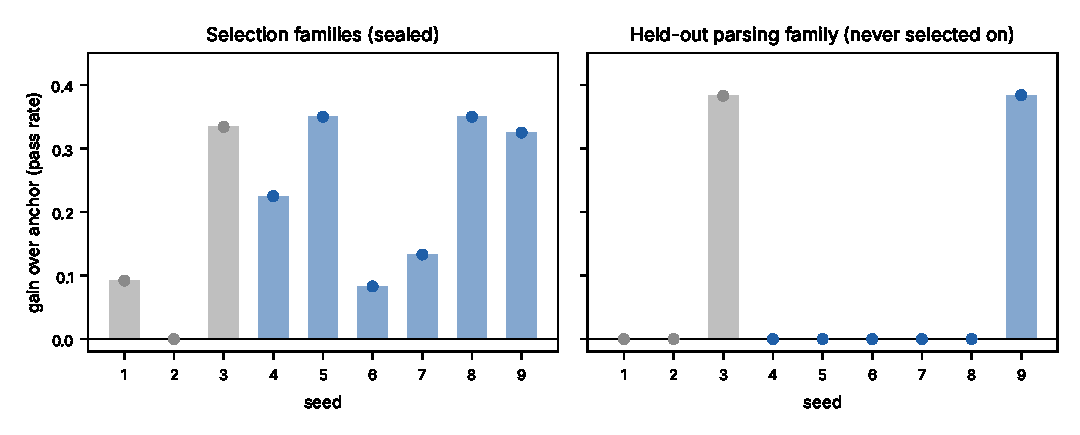
\includegraphics[width=0.95\linewidth]{docs/img/study3_seeds.pdf}
\caption{Per-seed gains over the anchor, for the selection families (left) and the held-out parsing family (right). Each bar is one run and its dot is the same value. Grey: suite v1 (seeds~1 to 3). Blue: suite v2 (seeds~4 to 9). Only seeds~3 and~9 have a nonzero held-out gain, and both are the \texttt{roman\_to\_int} fix.}
\label{fig:seeds}
\end{figure}

\paragraph{Repeatability.} All six replicates met the repeatability criterion, so $\ThrRepK$ of $6$ passed. The exact 95\% lower bound on that proportion is $\ThrRepLo$. The selection gains were $+0.225$, $+0.350$, $+0.083$, $+0.133$, $+0.350$, and $+0.325$. Their mean is $\ThrSelMean$ with a sample standard deviation of $\ThrSelSD$, and the 95\% $t$-interval is $[\ThrSelLo,\ThrSelHi]$. No final evaluation had a broken problem.

\paragraph{Transfer.} Held-out gains were $0$ in five replicates and $+0.384$ in seed~9. The mean is $\ThrHeldMean$ (sd $\ThrHeldSD$), with 95\% $t$-interval $[\ThrHeldLo,\ThrHeldHi]$. One of six replicates met the transfer criterion, which needs four, so the primary test is \emph{not met}. The exact 95\% interval for the transfer rate in the six replicates is $[\ThrTrLo,\ThrTrHi]$. Across all nine seeded runs, $\ThrTransferAllK$ of $9$ showed a held-out gain, with exact interval $[\ThrTrAllLo,\ThrTrAllHi]$.

\paragraph{Where the transfer comes from.} In both transfer runs (seeds~3 and~9), the model edited \texttt{roman\_to\_int} to implement the subtractive rule its docstring describes: \texttt{IV} is 4 and \texttt{IX} is 9. That function is in the held-out parsing family, so selection never saw it, and its fix carried over. The other two parsing tasks, \texttt{parse\_kv} and \texttt{caesar\_decode}, were not fixed in these runs. The parsing family has three tasks, so the transfer result rests on one of them.

\paragraph{Asymmetry.} Selection gain was positive in $\ThrSelPosAll$ of $9$ seeded runs, and the cross-family gap was positive in $\ThrGapPosAll$ of $9$. Seeds~3 and~9 have negative gaps, because their held-out gains are larger than their selection gains. The gap is the signature of overfitting that the held-out family was built to detect. Here it is positive in most runs, which is the pattern selection-only optimisation would produce. The two negative gaps are the runs that transferred.

\paragraph{Patch audits.} We read the patches behind the three observations that matter most: seed~3's \texttt{two\_sum} defect, the \texttt{roman\_to\_int} change in seeds~3 and~9, and the pilot's invalid accept. We have not audited every accepted patch. The rest of the accepted-patch set is part of the data still to be checked (Appendix~\ref{sec:repro}).

\section{Discussion and limitations}

\paragraph{What the study shows.} A live model that sees only source and docstrings produces accepted patches that are correct on fresh problems, and it did so in every pre-registered replicate. The gate did its job on the correctness path. The model's proposals are less predictable than a script's, and the gate still filtered them. We consider the judge's repair of D1 and the measurement of D2 the most useful outputs for the next study. Both defects were invisible to the pre-registered tests and became visible only by inspecting results.

\paragraph{What it does not show.} The primary test was not met. Generalisation rests on one function in one of fifteen tasks, in two of nine runs. We do not claim that the model transfers, and we do not claim that the kernel causes transfer. The held-out result is a property of this model on this task family.

\paragraph{Judge coverage.} The judge is only as good as its suite. D2 shows that a suite can pass a defect on most problems and still miss it on many. The residual gap depends on the defect family, and for the defect that occurred it is about \ThrMissLoopVtwo\%. Other docstring rules were not audited, so other defects may pass undetected. A judge that is not checked against each rule in its specification leaves room for the agent to satisfy the tests and miss the specification.

\paragraph{Reward hacking.} The defences are the sealed secret, the sandbox, the fresh batches, the coarse feedback, and the hash-chained ledger. None was stress-tested against an adversarial model, and we did not instruct the model to game the judge. No run had a security flag. This is evidence under a limited adversary, not a guarantee. The monitor that could have flagged overfitting ran in monitor mode, and we have not extracted its flags for every run. It should be enforced, or its status stated in every claim, before any stronger result is made.

\paragraph{Threats to validity.}
\begin{itemize}\setlength\itemsep{1pt}
\item \emph{Uncontrolled sampling.} LLM sampling is not seeded, and each replicate has its own secret. The replicates are independent folders, not controlled repeats.
\item \emph{Two suites.} Seeds~1 to 3 used v1 and seeds~4 to 9 used v2. The pre-registered sample is the second group.
\item \emph{Post-hoc deviations.} D1 and D2 were decided after results were seen. They are disclosed and written into the pre-registration.
\item \emph{One model, one provider.} All runs used \texttt{openai/gpt-oss-120b} through Groq. The model first chosen was retired by the provider during the study. Runs were executed on the author's machine, because the development sandbox's network policy blocked the provider.
\item \emph{Small tasks.} The suite has fifteen short functions, twelve in the selection families and three in the held-out family. The results say nothing about real repositories.
\item \emph{Cost.} The runs whose summaries we examined used between 7{,}920 and 10{,}977 model tokens each. We made no cost comparison with other approaches.
\item \emph{Judge semantics.} Patches are judged against docstrings, which are the specification. A wrong docstring can make a correct fix fail and a wrong fix pass.
\end{itemize}

\section{Related work}

Self-improving agents that rewrite their own code and validate changes empirically include the Darwin G\"odel Machine \citep{zhang2025dgm}, hyperagents, which make the improvement procedure itself editable \citep{zhang2026hyperagents}, and the Huxley--G\"odel Machine, which scores parents by their descendants' productivity \citep{wang2026hgm}. Formal foundations go back to \citet{schmidhuber2007godel}, and surveys cover the wider field \citep{chen2026rsi}.
Selecting the best of many patches on one distribution inflates the winner's score \citep{dwork2015holdout}. Proxy objectives are over-optimised under pressure \citep{gao2023scaling,coste2024ensembles}, and self-play judges can be convinced \citep{zhou2026convincing}.
Sequential and anytime-valid testing \citep{ramdas2023gtsavi,wald1945sprt} and online false-discovery control \citep{xu2024elond} underlie the gate. The kill rate of injected faults as a measure of test adequacy goes back to \citet{demillo1978mutation}.
Our contribution relative to these is the measurement: a live proposer behind a sealed, pre-registered judge, with its failures reported.

\section{Conclusion}

With a live model in the loop, the solver-only arm produces correct, gate-approved patches on fresh problems, in every pre-registered replicate. Transfer to the held-out family happened in two of nine runs through one docstring fix, which is too narrow to call generalisation.
The judge had two defects. D1 let a non-improvement through the gate, and it has been repaired. D2 is a coverage gap whose size depends on the bug. We now know how big the gap is for the defect that occurred, and that another suite is needed before the improver arm is run.

\paragraph{Next step.} Study~4 asks whether the loop can improve the code that proposes and judges its own changes. The design, the guard, and the open decisions are in \texttt{study4/}. The guard refuses to run without a locked pre-registration, and none has been locked. Study~4 will not start until the judge covers every rule in its specification, or states which rules it does not cover.

\paragraph{Reproducibility.} Code and data: \repo. Tests: \texttt{python -m pytest -q tests} (131 tests at the final commit). Suite detection: \texttt{python results/study3/suite\_detection.py}. All statistics, macros, tables and the figure in this paper: \texttt{python results/study3/make\_study3\_paper.py}, which reads \texttt{results/study3/seed\_summary.json} and \texttt{results/study3/suite\_detection.json}. Study~2 is reproduced by \texttt{python run\_study2.py check}.

\paragraph{Disclosure.} Substantial AI assistance was used to write the code and to draft this paper. The author chose the design and is responsible for the content. Numbers come from generated files or from the run summaries listed in Appendix~\ref{sec:repro}. References marked FROM-KNOWLEDGE in \texttt{references.bib} were not re-fetched.

\bibliographystyle{plainnat}
\bibliography{references}

\appendix
\section{Pre-registration timeline and deviations}
\label{app:timeline}

The order of events was as follows. The first live pilot ran with the buggy utility path (D1), and its cycle-0 accept was found afterwards. The gate was fixed (commit \texttt{68d3517}) before any replicate ran. Seed~0 and seeds~1 to 3 were run under suite v1. Seed~3's \texttt{two\_sum} defect was then found, and suite v2 was added (commit \texttt{7e5b697}). The six-seed design, under v2, was written into the pre-registration before seeds~4 to 9 ran. The pre-registration file is \texttt{results/study3/prereg.json}, with body hash \texttt{634c1f4c}, and it lists D1 and D2 as deviations.
Both deviations are post hoc. At the final commit, the three code files named in the pre-registration (\texttt{run\_study3\_live.py}, \texttt{kernel/llm\_meta.py}, \texttt{study3\_summary.py}) match their recorded hashes, so none of them has changed since the pre-registration was written. The pilot and the smoke run are reported, but they are not part of the verdicts.

\section{Data availability and reproduction}
\label{sec:repro}

\paragraph{What is in the repository.} The seed-level gains, broken counts, and per-run anchors for seeds~1 to 3 (\texttt{results/study3/seed\_summary.json}), the detection measurements (\texttt{results/study3/suite\_detection.json}), the pre-registration, the deviation record, and the scripts that produce every number and figure here.
\paragraph{What is not yet in the repository.} The per-run anchors, final pass rates, accept counts and cycle-by-cycle ledgers for seeds~4 to 9, and the full set of accepted patches for every run. These are in the run folders, which were produced on the author's machine and are not committed. They must be added before submission, and the gaps in Table~\ref{tab:seeds} must then be filled.

\paragraph{Commands.}
\begin{verbatim}
python results/study3/suite_detection.py        # Table 1
python results/study3/make_study3_paper.py      # every other number, table and figure
python -m pytest -q tests                       # 131 tests
python run_study3_live.py --cycles 3 --seed 4 --out runs/study3_seed4   # one live replicate
python study3_summary.py runs/study3_seed4      # per-run summary and verdicts
\end{verbatim}
A live replicate needs \texttt{GROQ\_API\_KEY} in the environment. The key is never written to a file. Replicates must not set \texttt{SI\_LOOP\_SECRET}, which would give every folder the same secret.

\end{document}
